%=========================================================================
% Start of
%=========================================================================
\preClass{Operations on Functions}

\begin{problem}
\item A restaurant would like to test a new menu item. They estimate
  that the cost for producing $x$ servings in market A is 12\$ per
  serving. They estimate that the cost for producing $y$ servings in
  market B is \$15 per serving.  They will allocate a total of
  \$36,000 for producing the total number of servings. Write out an
  expression that relates the cost of the number of servings produced
  in market A and market B.
  \vfill
\item The number of mosquitoes per acre in an area is estimated to be
  600 times the area of open water measured in acres. The area of open
  water in a location is declining over time and is
  $A(t)=50-\frac{1}{3}t$, where $t$ is the number of years since
  January 1 of the current year. Determine the number of mosquitoes
  per acre in terms of $t$.
  \vfill
\item The delay time required for a neuron to recharge is estimate to
  be a function of the calcium concentration,
  \begin{eqnarray*}
    \mathrm{Recharge([Ca])} & = & 0.05-\mathrm{[Ca]}^2.
  \end{eqnarray*}
  The concentration of calcium in an experiment is changed over time
  and is estimated to be
  \begin{eqnarray*}
    \mathrm{[Ca]}(t) & = & 0.01+\frac{1}{1+t}.
  \end{eqnarray*}
  Determine the formula used to estimate the recharge delay as a
  function of time, $t$. \textit{(Do not simplify the expression.)}
  \vfill
\end{problem}


\actTitle{Operations on Functions}
\begin{problem}
\item A function is defined to be
  \begin{eqnarray*}
    f(x) & = & x^2.
  \end{eqnarray*}
  Determine the value of $a$ and $b$ so that the function
  \begin{eqnarray*}
    g(x) & = & f(x-a)+b
  \end{eqnarray*}
  is the original function that is shifted up two units and left 3
  units. Plot the graphs of $f(x)$ and $g(x)$ on the coordinate plane below.

  \begin{tikzpicture}[y=1.1cm, x=1.1cm,font=\sffamily]
      % bounds
      \def\lowX{-5.5}
      \pgfmathtruncatemacro\startX{round(0.5+\lowX)}
      \pgfmathsetmacro\nextXValue{int(\startX+1)}
      \def\highX{5.5}
      \def\lowY{-5.5}
      \def\highY{5.5}
      \pgfmathsetmacro\nextYValue{int(\lowY+1)}
      % ticks
      \draw[step = 1, gray, very thin,dashed,opacity=0.85] (\lowX, \lowY) grid ( \highX,\highY);
    % axis
    \draw[thick,->] (\lowX,0) -- coordinate (x axis mid) (\highX,0) node[anchor = north west] {$x$};
      \draw[thick,->] (0,\lowY) -- coordinate (y axis mid) (0,\highY) node[anchor = north east] {$y$};
      \foreach \y in {-5,-4,...,-1,1,2,...,\highY} {
        \draw (1pt, \y) -- (-1pt, \y) node[yshift=-6,xshift=-1,anchor=east] {$\y$};
      }
      \foreach \x in {-5,-4,...,-1,1,2,...,\highX} {
        \draw (\x,1pt) -- (\x,-1pt) node[yshift=-5,xshift=-1,anchor=east] {$\x$};
      }
      \draw (0,5.5) node [anchor=south] {Comparing Shifted Functions};
    \end{tikzpicture}

  \clearpage

\item Two functions are given in the tables below.

  \begin{tabular}[h]{l||l|l|l|l|l}
    $x$    & 0 & 1 & 2 & 3 & 4 \\ \hline
    $f(x)$ & a & m & k & a & h \\
  \end{tabular}

  \begin{tabular}[h]{l||l|l|l|l|l}
    $x$    & a & c & h & j & m \\ \hline
    $g(x)$ & $\natural$ & $\Diamond$ & $\Box$ & $\heartsuit$ & $\Diamond$ \\
  \end{tabular}

  \begin{subproblem}
  \item Determine the range and domain of $f$.
    \vspace{2em}
  \item Determine the range and domain of $g$.
    \vspace{2em}
  \item Determine the values of each of the following expressions:
    \begin{eqnarray*}
      f(2) & = & \\
      f(4) & = & \\
      g(f(2)) & = & \\
      g(f(1)) & = & \\
      g(f(0))+g(f(3)) & = &
    \end{eqnarray*}
  \item If $f(x)=$h what is the value of $x$?
  \end{subproblem}

  \clearpage

\item The expected amount in insurance claims, $I$, for a small,
  college town depends on the number, $N$, of outside visitors to the
  town, and the graph of the relationship is shown in the plot on the
  left below. The number of visitors changes over the course of a
  week, and the number of visitors based on the day of the week is
  shown in the graph on the right. (Zero corresponds to Sunday.)

  \hspace{-7em}
  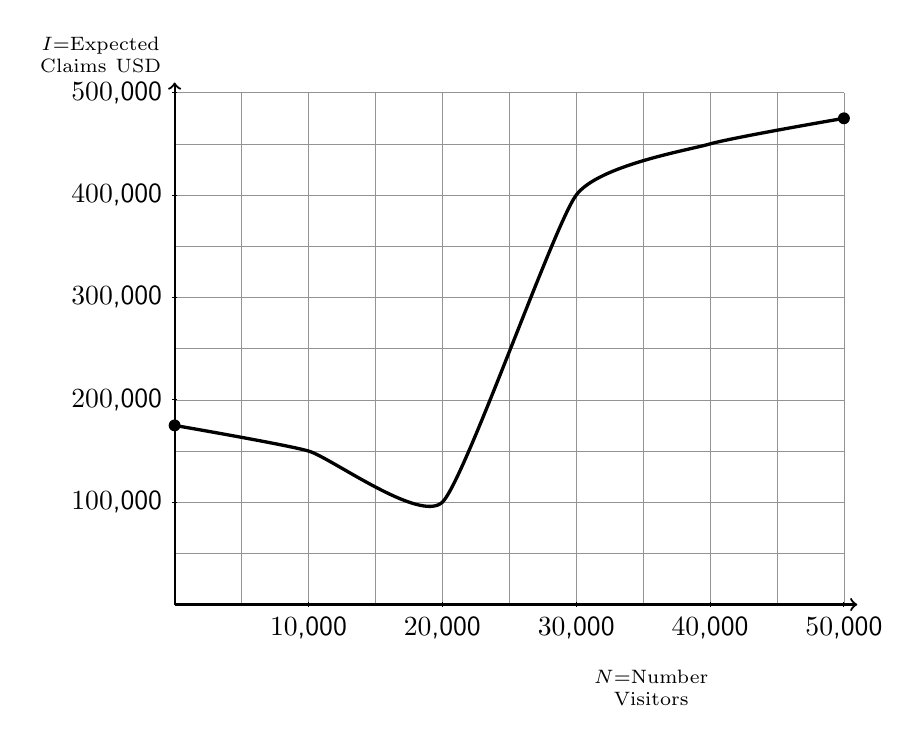
\begin{tikzpicture}[y=0.13mm, x=1.7mm,font=\sffamily]
    % ticks
    \draw[xstep = 5,ystep=50, gray, very thin,opacity=0.85] (0, 0) grid (50, 500);
 	% axis
	\draw[thick,->] (0,0) -- coordinate (x axis mid) (51,0) 
          node[yshift=-2em,xshift=-10em,anchor = north west] {$N=\mathrm{Number}\atop\mathrm{Visitors}$};
    \draw[thick,->] (0,0) -- coordinate (y axis mid) (0,510) 
          node[anchor = south east] {$I=\mathrm{Expected}\atop\mathrm{Claims~USD}$};
    \foreach \y in {100,200,300,400,500} {
      \draw (1pt, \y) -- (-1pt, \y) node[anchor = east] {$\y$,000};
    }
    \foreach \x in {10,20,...,50} {
      \draw (\x,1pt) -- (\x,-1pt) node[anchor = north] {$\x$,000};
    }
    % Draw the function
    \draw [black, very thick] plot [smooth, tension=0.3] coordinates {
      (0,175) (10,150) (20,100) (30,400) (40,450) (50,475)};
    \fill[black] (0, 175)  circle [radius=0.5ex];
    \fill[black] (50,475) circle [radius=0.5ex];
  \end{tikzpicture}
  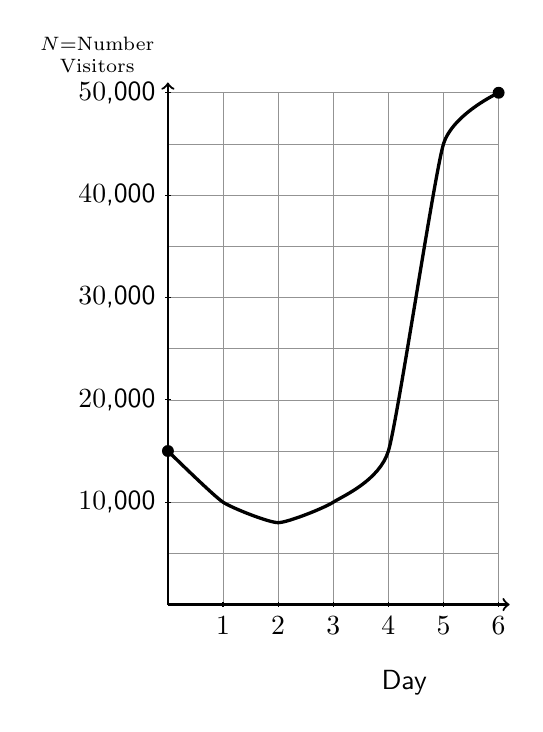
\begin{tikzpicture}[y=1.3mm, x=7.0mm,font=\sffamily]
    % ticks
    \draw[xstep = 1,ystep=5, gray, very thin,opacity=0.85] (0, 0) grid (6, 50);
 	% axis
	\draw[thick,->] (0,0) -- coordinate (x axis mid) (6.2,0) 
          node[yshift=-2em,xshift=-5em,anchor = north west] {Day};
    \draw[thick,->] (0,0) -- coordinate (y axis mid) (0,51) 
          node[anchor = south east] {$N=\mathrm{Number}\atop\mathrm{Visitors}$};
    \foreach \y in {10,20,30,40,50} {
      \draw (1pt, \y) -- (-1pt, \y) node[anchor = east] {$\y$,000};
    }
    \foreach \x in {1,2,...,6} {
      \draw (\x,1pt) -- (\x,-1pt) node[anchor = north] {$\x$};
    }
    % Draw the function
    \draw [black, very thick] plot [smooth, tension=0.3] coordinates {
      (0,15) (1,10) (2,8) (3,10) (4,15) (5,45) (6,50)};
    \fill[black] (0, 15)  circle [radius=0.5ex];
    \fill[black] (6,50) circle [radius=0.5ex];
  \end{tikzpicture}

  \begin{subproblem}
  \item What is the expected amount of insurance claims on Monday?
    \vfill
  \item As the day of the week increases from Sunday to Monday what is
    the change in the expected insurance claims?
    \sideNote{A negative number indicates a decrease, and a positive
      number indicates an increase.}
    \vfill
  \item As the day of the week increases from Wednesday to Thursday
    what is the change in the expected insurance claims?
    \vfill
  \item Explain what meaning the expression $I(N(d))$ has where $d$ is
    the day of the week.
    \vfill
  \item How can the function $I(N(d))$ increase from Sunday to Monday
    when both functions are decreasing?
    \vspace{1em}
  \end{subproblem}

\clearpage

\item The owner of a shop will be selling two similar items and hopes
  that customers will choose to buy either one or the other of these
  items. The products are about the same size, and each one will take
  up about 0.5 m\textsuperscript{2} of space. The first item will be
  sold for 10\$ each, and the second item will be sold for 12\$
  each. The cost to the owner depends on how many the owner buys,
  \begin{eqnarray*}
    C_1(x) & = & 5 - \frac{1}{20}(x-10)^2, \\
    C_2(y) & = & 5 - \frac{1}{20}(y-10)^2,
  \end{eqnarray*}
  where $x$ is the number of the first item sold, and $y$ is the
  number of the second item sold.

%The owner has allocated 1000\$ for the two products and has 35
%  m\textsuperscript{2} of total space for the two items.  The owner
%  will buy $x$ units of the first item and $y$ units of the second
%  item.

  \begin{subproblem}
    
  \item Determine the relationship that determines the total revenue
    for selling the two items. (Revenue is the total amount of sales.)

    \vfill

  \item Determine the relationship that determines the total cost for
    selling the items.

    \vfill

  \item Make a sketch of the graphs of the two relationships. Use the
    left axes for the revenue, and use the right axes for the cost.

  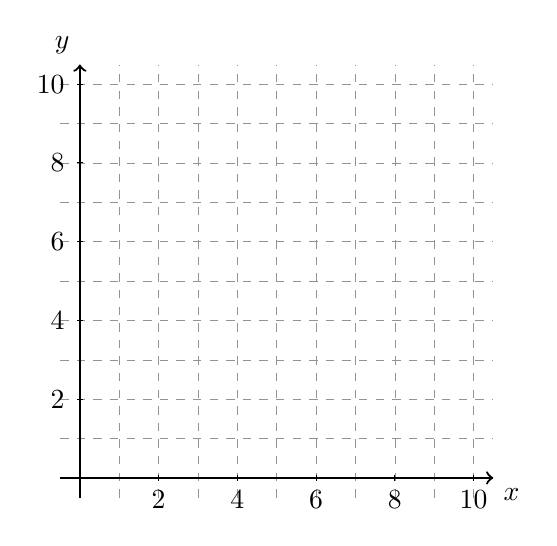
\begin{tikzpicture}[y=0.5cm, x=0.5cm,font=\sffamily]
      % bounds
      \def\lowX{-0.5}
      \pgfmathtruncatemacro\startX{round(0.5+\lowX)}
      \pgfmathsetmacro\nextXValue{int(\startX+1)}
      \def\highX{10.5}
      \def\lowY{-0.5}
      \def\highY{10.5}
      \pgfmathsetmacro\nextYValue{int(\lowY+1)}
      % ticks
      \draw[step = 1, gray, very thin,dashed,opacity=0.85] (\lowX, \lowY) grid ( \highX,\highY);
    % axis
    \draw[thick,->] (\lowX,0) -- coordinate (x axis mid) (\highX,0) node[anchor = north west] {$x$};
      \draw[thick,->] (0,\lowY) -- coordinate (y axis mid) (0,\highY) node[anchor = south east] {$y$};
      \foreach \y in {2,4,...,\highY} {
        \draw (1pt, \y) -- (-1pt, \y) node[yshift=-0,xshift=-1,anchor=east] {$\y$};
      }
      \foreach \x in {2,4,...,\highX} {
        \draw (\x,1pt) -- (\x,-1pt) node[yshift=-0,xshift=-0,anchor=north] {$\x$};
      }
    \end{tikzpicture}
  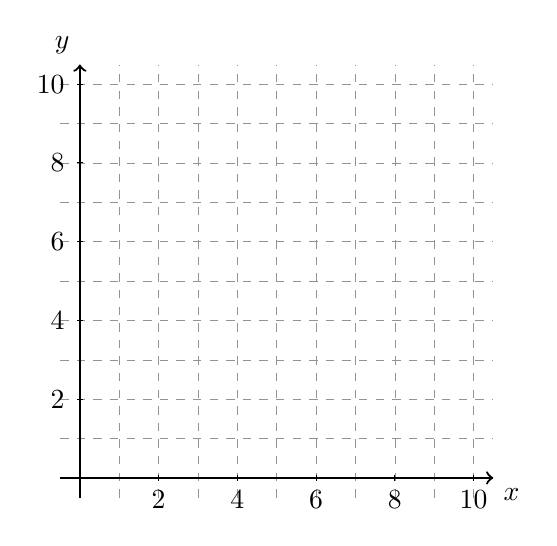
\begin{tikzpicture}[y=0.5cm, x=0.5cm,font=\sffamily]
      % bounds
      \def\lowX{-0.5}
      \pgfmathtruncatemacro\startX{round(0.5+\lowX)}
      \pgfmathsetmacro\nextXValue{int(\startX+1)}
      \def\highX{10.5}
      \def\lowY{-0.5}
      \def\highY{10.5}
      \pgfmathsetmacro\nextYValue{int(\lowY+1)}
      % ticks
      \draw[step = 1, gray, very thin,dashed,opacity=0.85] (\lowX, \lowY) grid ( \highX,\highY);
    % axis
    \draw[thick,->] (\lowX,0) -- coordinate (x axis mid) (\highX,0) node[anchor = north west] {$x$};
      \draw[thick,->] (0,\lowY) -- coordinate (y axis mid) (0,\highY) node[anchor = south east] {$y$};
      \foreach \y in {2,4,...,\highY} {
        \draw (1pt, \y) -- (-1pt, \y) node[yshift=-0,xshift=-1,anchor=east] {$\y$};
      }
      \foreach \x in {2,4,...,\highX} {
        \draw (\x,1pt) -- (\x,-1pt) node[yshift=-0,xshift=-0,anchor=north] {$\x$};
      }
    \end{tikzpicture}

  \item If the owner chooses to purchase 4 of the first item,
    determine the total profit. (Assume everything is sold.)
    \vfill

  \item Determine the function that represents the total profit given
    the number of the first item purchased by the owner. (Assume
    everything is sold.)
    \vfill

  \end{subproblem}

  \clearpage


\end{problem}

\postClass

\begin{problem}
\item Briefly state two ideas from today's class.
  \begin{itemize}
  \item
  \item
  \end{itemize}

\item Two functions are given in the tables below.

  \begin{tabular}[h]{l||l|l|l|l|l}
    $x$    & 0 & 1 & 2 & 3 & 4 \\ \hline
    $f(x)$ & a & m & k & a & h \\
  \end{tabular}

  \begin{tabular}[h]{l||l|l|l|l|l}
    $x$    & a & c & h & j & m \\ \hline
    $g(x)$ & $\natural$ & $\Diamond$ & $\Box$ & $\heartsuit$ & $\Diamond$ \\
  \end{tabular}

  \begin{subproblem}
  \item If $g(f(x))=\natural$ what are the possible values of $x$? Is
    this reverse procedure a function?
  \item If $g(x)=\Diamond$ what are the possible values of $x$? Is
    this reverse procedure a function?
  \item Express the function $g(f(x))$ as a table.
  \item Determine the range and domain of $g(f(x))$.
  \end{subproblem}

  \clearpage

\item Two functions are shown in the figure below. The function
  plotted with the dotted line is $f(x)$, and the function plotted
  with the solid line is $g(x)$. Express $g(x)$ in terms of $f(x)$,
  \begin{eqnarray*}
    g(x) & = &
  \end{eqnarray*} \\
  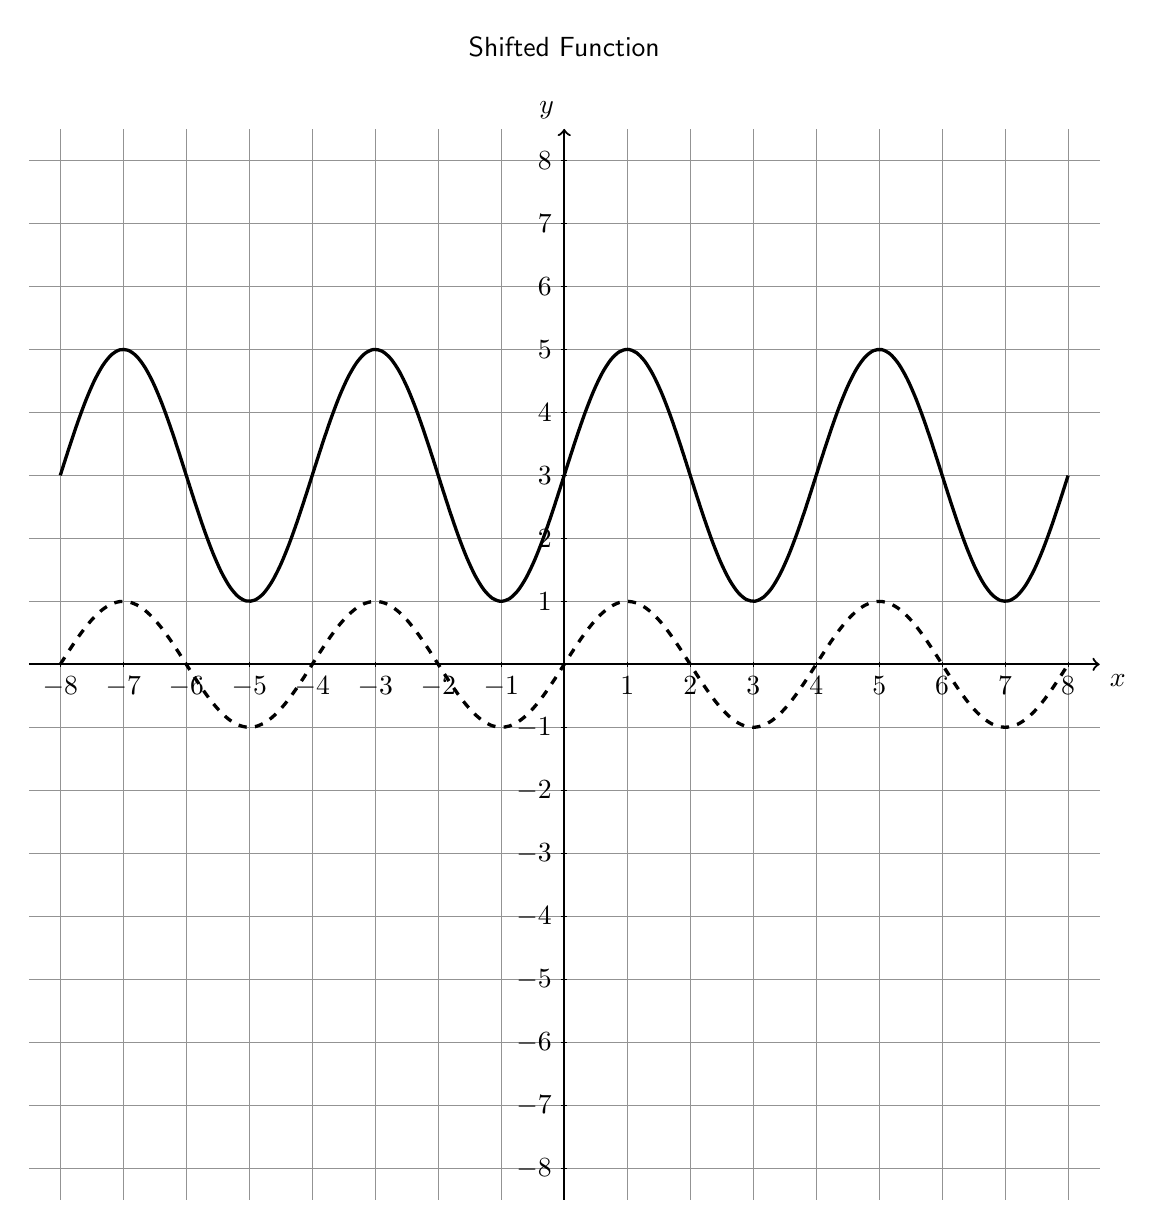
\begin{tikzpicture}[y=0.8cm, x=0.8cm,font=\sffamily]
  % Define the x bounds
  \def\lowX{-8.5}
  \pgfmathtruncatemacro\startX{round(0.5+\lowX)}
  \def\highX{8.5}
  \pgfmathtruncatemacro\endX{round(\highX-0.5)}
  % define the y bounds
  \def\lowY{-8.5}
  \pgfmathtruncatemacro\startY{round(0.5+\lowY)}
  \def\highY{8.5}
  \pgfmathtruncatemacro\endY{round(\highY-0.5)}
  % Add a grid
  \draw[step = 1, gray, very thin,opacity=0.85] (\lowX, \lowY) grid ( \highX, \highY);
% Draw the axes
\draw[thick,->] (\lowX,0) -- coordinate (x axis mid) (\highX,0) node[anchor = north west] {$x$};
  \draw[thick,->] (0,\lowY) -- coordinate (y axis mid) (0,\highY) node[anchor = south east] {$y$};
  % Label the y axis
  \pgfmathsetmacro\nextYValue{int(\startY+1)}
  \foreach \y in {\startY,\nextYValue,...,-1,1,2,...,\highY} {
    \draw (1pt, \y) -- (-1pt, \y) node[anchor = east] {$\y$};
  }
  % Label the x axis
  \pgfmathsetmacro\nextXValue{int(\startX+1)}
  \foreach \x in {\startX,\nextXValue,...,-1,1,2,...,\endX} {
    \draw (\x,1pt) -- (\x,-1pt) node[anchor = north] {$\x$};
  }
  % Draw the function.
  \begin{scope}
    %\clip(-4,-1) rectangle (8,5);
    \draw[scale=1.0,domain=\startX:\endX,smooth,variable=\x,very thick,black,samples=120]
         plot ({\x},{3+2*sin(deg(pi*\x/2))});
     \draw[scale=1.0,domain=\startX:\endX,smooth,variable=\x,very thick,dashed,black,samples=120]
        plot ({\x},{sin(deg(pi*\x/2))});
  \end{scope}

  %\node[above=0.1cm] at (-2,2 )   {\nextXValue};
  \draw (0,9.5) node [anchor=south] {Shifted Function};

\end{tikzpicture}

\clearpage

\item Two functions are shown in the figure below. The function
  plotted with the dotted line is $f(x)$, and the function plotted
  with the solid line is $g(x)$. Express $g(x)$ in terms of $f(x)$.
  \begin{eqnarray*}
    g(x) & = &
  \end{eqnarray*} \\
  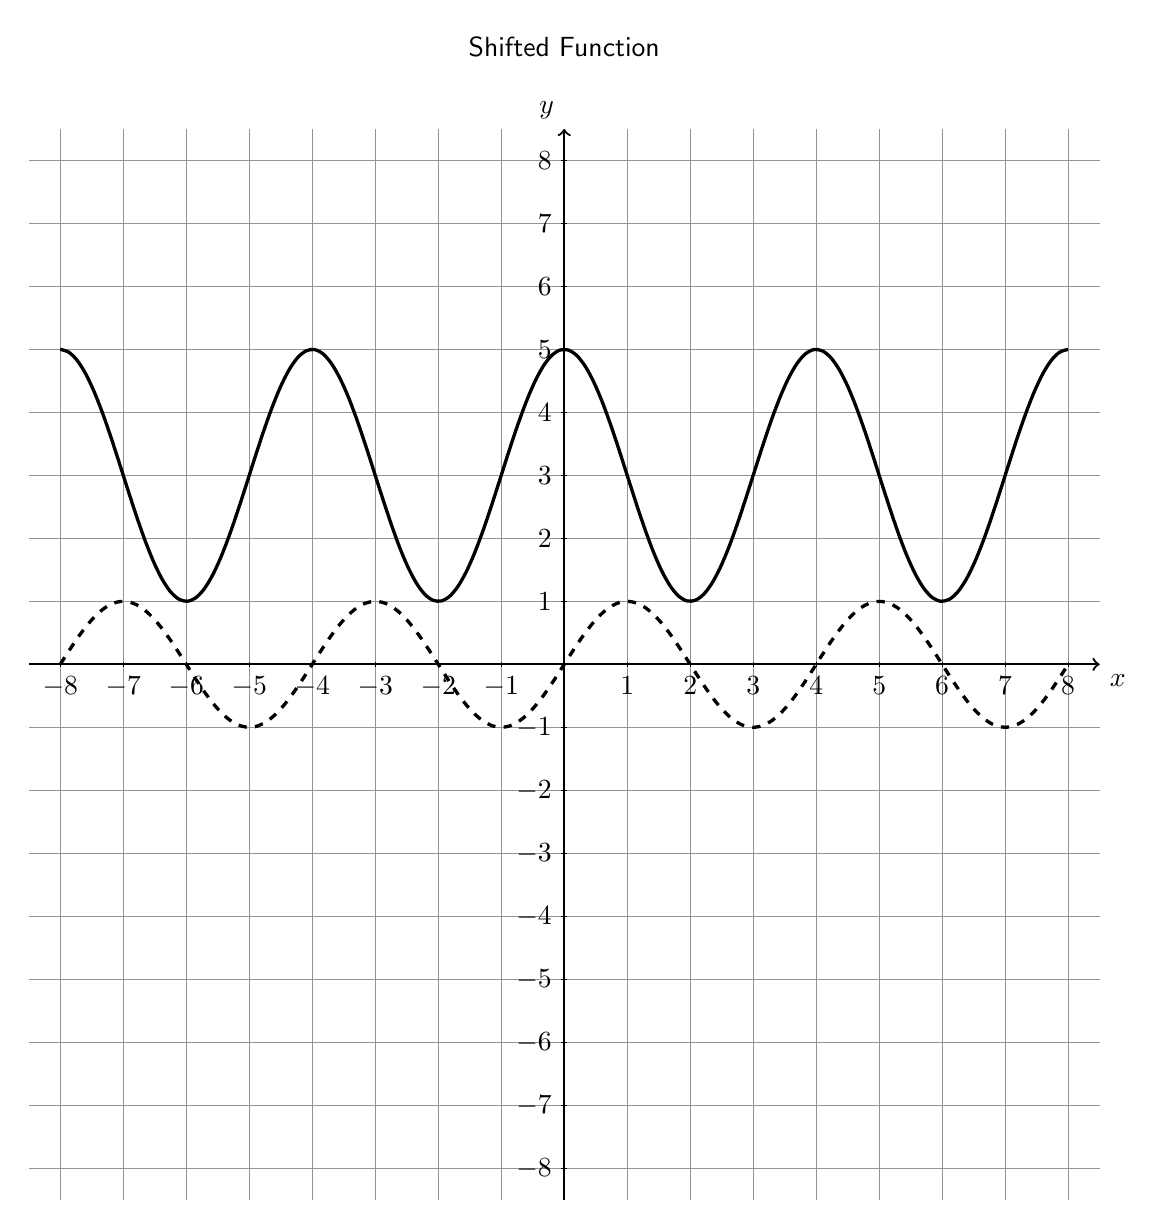
\begin{tikzpicture}[y=0.8cm, x=0.8cm,font=\sffamily]
  % Define the x bounds
  \def\lowX{-8.5}
  \pgfmathtruncatemacro\startX{round(0.5+\lowX)}
  \def\highX{8.5}
  \pgfmathtruncatemacro\endX{round(\highX-0.5)}
  % define the y bounds
  \def\lowY{-8.5}
  \pgfmathtruncatemacro\startY{round(0.5+\lowY)}
  \def\highY{8.5}
  \pgfmathtruncatemacro\endY{round(\highY-0.5)}
  % Add a grid
  \draw[step = 1, gray, very thin,opacity=0.85] (\lowX, \lowY) grid ( \highX, \highY);
% Draw the axes
\draw[thick,->] (\lowX,0) -- coordinate (x axis mid) (\highX,0) node[anchor = north west] {$x$};
  \draw[thick,->] (0,\lowY) -- coordinate (y axis mid) (0,\highY) node[anchor = south east] {$y$};
  % Label the y axis
  \pgfmathsetmacro\nextYValue{int(\startY+1)}
  \foreach \y in {\startY,\nextYValue,...,-1,1,2,...,\highY} {
    \draw (1pt, \y) -- (-1pt, \y) node[anchor = east] {$\y$};
  }
  % Label the x axis
  \pgfmathsetmacro\nextXValue{int(\startX+1)}
  \foreach \x in {\startX,\nextXValue,...,-1,1,2,...,\endX} {
    \draw (\x,1pt) -- (\x,-1pt) node[anchor = north] {$\x$};
  }
  % Draw the function.
  \begin{scope}
    %\clip(-4,-1) rectangle (8,5);
    \draw[scale=1.0,domain=\startX:\endX,smooth,variable=\x,very thick,black,samples=120]
         plot ({\x},{3+2*sin(deg(pi*\x/2+pi/2))});
     \draw[scale=1.0,domain=\startX:\endX,smooth,variable=\x,very thick,dashed,black,samples=120]
        plot ({\x},{sin(deg(pi*\x/2))});
  \end{scope}

  %\node[above=0.1cm] at (-2,2 )   {\nextXValue};
  \draw (0,9.5) node [anchor=south] {Shifted Function};

\end{tikzpicture}

  Add a sketch of the graph of the function $h(x)=3f(x+2)-5$ to the plot above.

  Can you find a different formula whose graph looks exactly the same as $g(x)$?


\end{problem}


%%% Local Variables:
%%% mode: latex
%%% TeX-master: "../labManual"
%%% End:
